\documentclass{cmn}
\usetikzlibrary{decorations.markings}

\newlength\width
\setlength\width{9mm}
\newlength\height
\setlength\height{6mm}

\begin{document}
  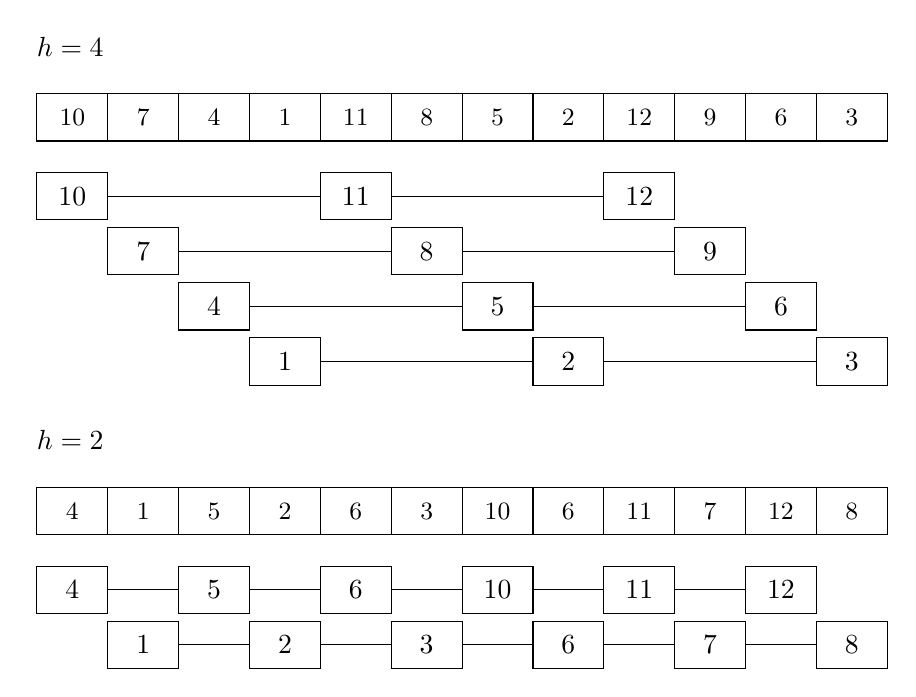
\begin{tikzpicture}
    \begin{scope}
      \node[text width=10mm,align=left] at (5mm,12mm) {$h=4$};

      % top cells
      \draw (0,0) -- ++(12*\width,0) -- ++(0,\height) -- ++(-12*\width,0) -- cycle;
      \foreach[count=\i] \n in {10,7,4,1,11,8,5,2,12,9,6,3} {
        \node at (\i*\width-\width/2,\height/2) {\small $\n$};
      }
      \foreach \i in {1,...,11} {
        \draw (\i*\width,0) -- ++(0,\height);
      }

      % bottom cells
      \foreach \i in {0,...,2} {
        \foreach \j in {0,...,3} {
          \pgfmathtruncatemacro\n{10+\i-3*\j}
          \pgfmathtruncatemacro\x{\i*4+\j}
          \pgfmathsetmacro\y{-10-\j*7}

          % cell
          \draw (\x*\width,\y mm) -- ++(\width,0) -- ++(0,\height) -- ++(-\width,0) -- cycle;

          \node at (\x*\width+\width/2,\y mm + \height/2) {\n};
        }
      }

      % bottom lines
      \foreach \i in {0,...,1} {
        \foreach \j in {0,...,3} {
          \pgfmathtruncatemacro\x{\i*4+\j+1}
          \pgfmathsetmacro\y{-10-\j*7}

          \draw (\x*\width,\y mm + \height/2) -- ++(3*\width,0);
        }
      }
    \end{scope}

    \begin{scope}[yshift=-50mm]
      \node[text width=10mm,align=left] at (5mm,12mm) {$h=2$};

      % top cells
      \draw (0,0) -- ++(12*\width,0) -- ++(0,\height) -- ++(-12*\width,0) -- cycle;
      \foreach[count=\i] \n in {4,1,5,2,6,3,10,6,11,7,12,8} {
        \node at (\i*\width-\width/2,\height/2) {\small $\n$};
      }
      \foreach \i in {1,...,11} {
        \draw (\i*\width,0) -- ++(0,\height);
      }

      % bottom cells (odd)
      \foreach[count=\i] \n in {4,5,6,10,11,12} {
        \pgfmathtruncatemacro\x{\i*2}
        \pgfmathsetmacro\y{-10}

        % cell
        \draw (\x*\width-2*\width,\y mm) -- ++(\width,0) -- ++(0,\height) -- ++(-\width,0) -- cycle;

        \node at (\x*\width-3*\width/2,\y mm + \height/2) {\n};
      }

      % bottom cells (even)
      \foreach[count=\i] \n in {1,2,3,6,7,8} {
        \pgfmathtruncatemacro\x{\i*2+1}
        \pgfmathsetmacro\y{-10-7}

        % cell
        \draw (\x*\width-2*\width,\y mm) -- ++(\width,0) -- ++(0,\height) -- ++(-\width,0) -- cycle;

        \node at (\x*\width-3*\width/2,\y mm + \height/2) {\n};
      }

      % bottom lines
      \foreach \i in {0,...,4} {
        \foreach \j in {0,1} {
          \pgfmathtruncatemacro\x{\i*2+\j+1}
          \pgfmathsetmacro\y{-10-\j*7}

          \draw (\x*\width,\y mm + \height/2) -- ++(\width,0);
        }
      }
    \end{scope}
  \end{tikzpicture}
\end{document}
